\documentclass{article}
%Preamble
\usepackage{float}
\usepackage{color}
\usepackage{listings}
\usepackage{longtable}
\usepackage{amsmath,amssymb}
\usepackage{graphics}
\usepackage{graphicx}

\title{AE 625 -Particle Methods in Fluid Flow Simulation \\ Assignment 5: Report }
\author{Aditi Taneja}
\date{}

%Preamble
%\usepackage{graphicx}
\begin{document}
\pagenumbering{arabic}
\maketitle

\begin{figure}[H]   \label{figure}
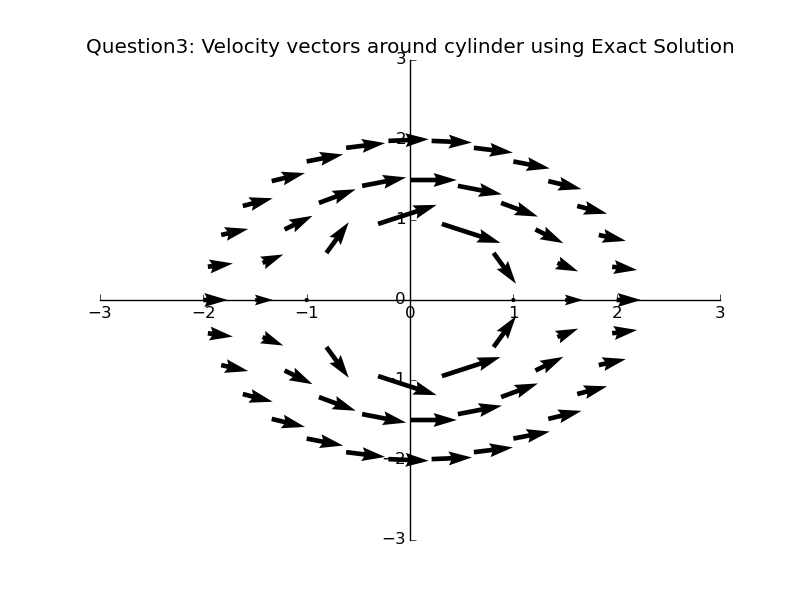
\includegraphics[width=12cm]{velocity_plot_exact.png}
\caption{Velocity Distribution around Cylinder from Exact Solution}
\label{figure:}
\end{figure}

\begin{figure}[H] \label{figure}
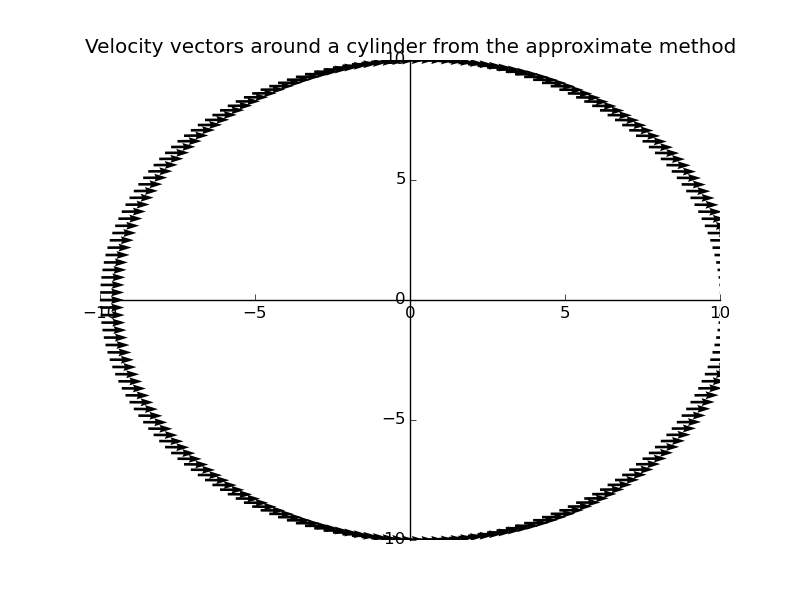
\includegraphics[width=12cm]{approx_q1.png}
\caption{Velocity Distribution around Cylinder from Panel Method Approximation}
\label{figure:}
\end{figure}

\begin{figure}[H] \label{figure}
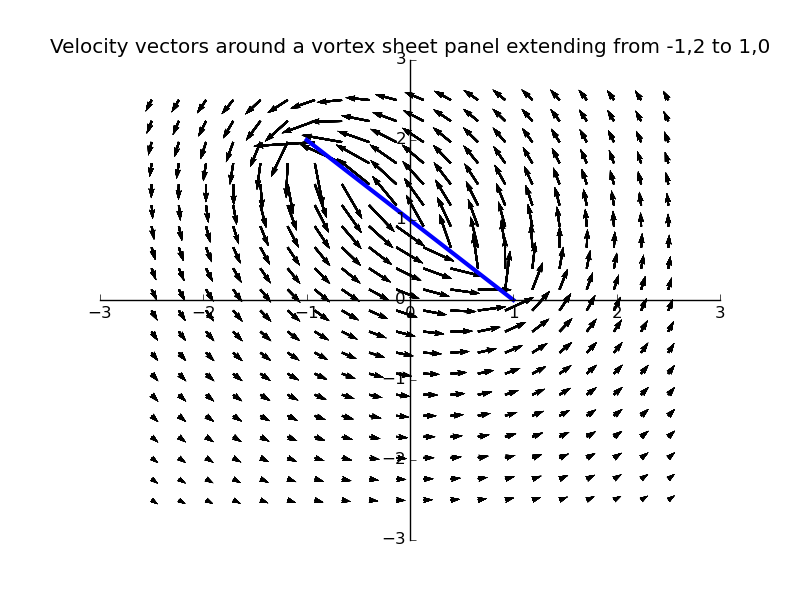
\includegraphics[width=12cm]{panel.png}
\caption{Velocity Distribution around Panel inclined at 45 degrees and length = 2.0 }
\label{figure:}
\end{figure}

\begin{figure}[H] \label{figure}
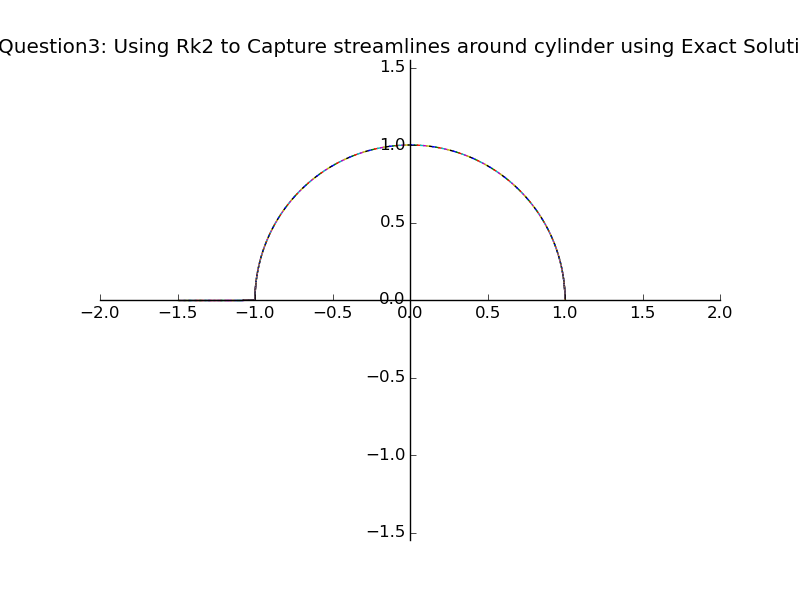
\includegraphics[width=12cm]{streamline_exact.png}
\caption{Streamline around Cylinder With Free stream velocity = 1.0}
\label{figure:}
\end{figure}

\begin{figure}[H] \label{figure}
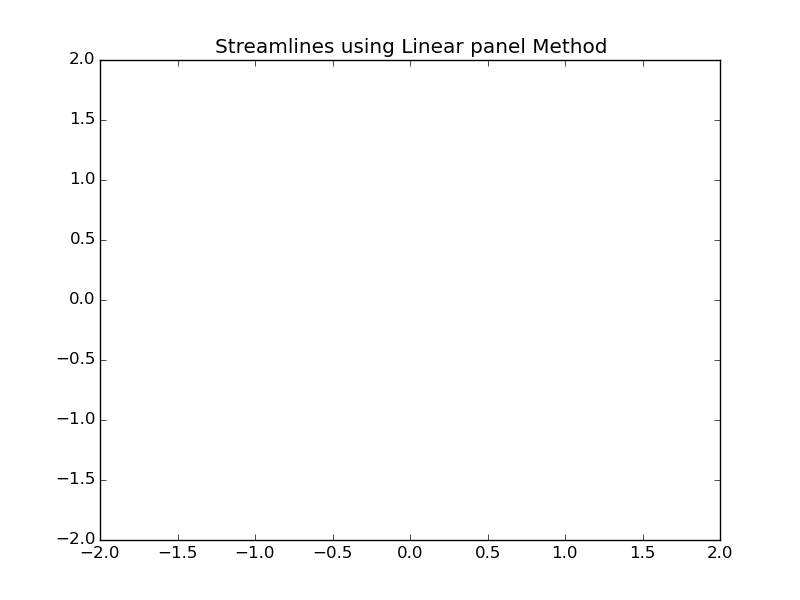
\includegraphics[width=12cm]{streamlines.png}
\caption{Streamlines around Cylinder using linear panel method with Free stream velocity = 1.0}
\label{figure:}
\end{figure}

\newpage
\section*{Question1}
Consider a ring of points (say 200) at a radius R outside the cylinder (i.e. R>1), vary R and plot the average error in the value of the velocity magnitued with the exact solution.

\begin{figure}[H]  \label{figure}
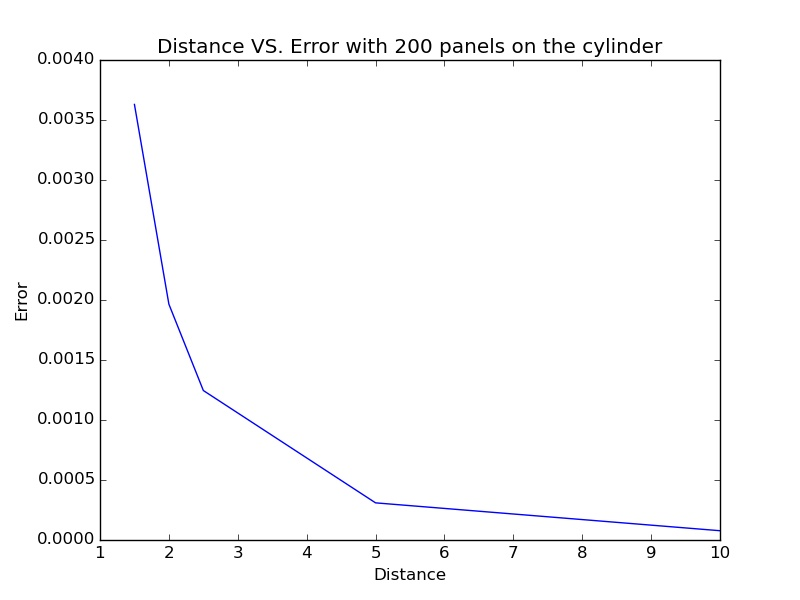
\includegraphics[width=12cm]{result1.jpg}
\caption{Error(relative average) Vs. Distance assuming 200 panels on the cylinder}
\label{figure:}
\end{figure}

\newpage
\section*{Question 2}
Do part 1 for different number of panels (say 20 to 100 or more).
\\
Plots obtained for Panels 20,100,500:
\begin{figure}[H] \label{figure}
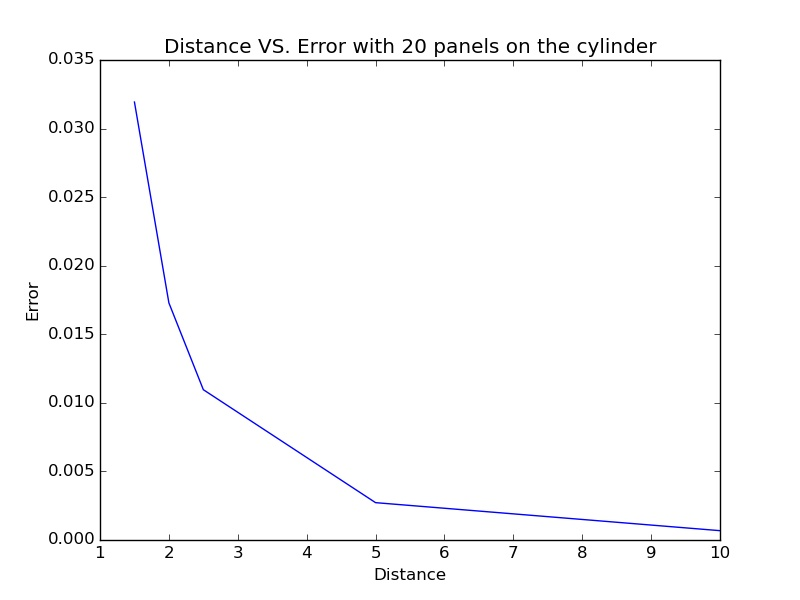
\includegraphics[width=12cm]{result2.jpg}
\caption{Error(relative average) Vs. Distance assuming 20 panels on the cylinder}
\label{figure:}
\end{figure}

\begin{figure}[H]  \label{figure}
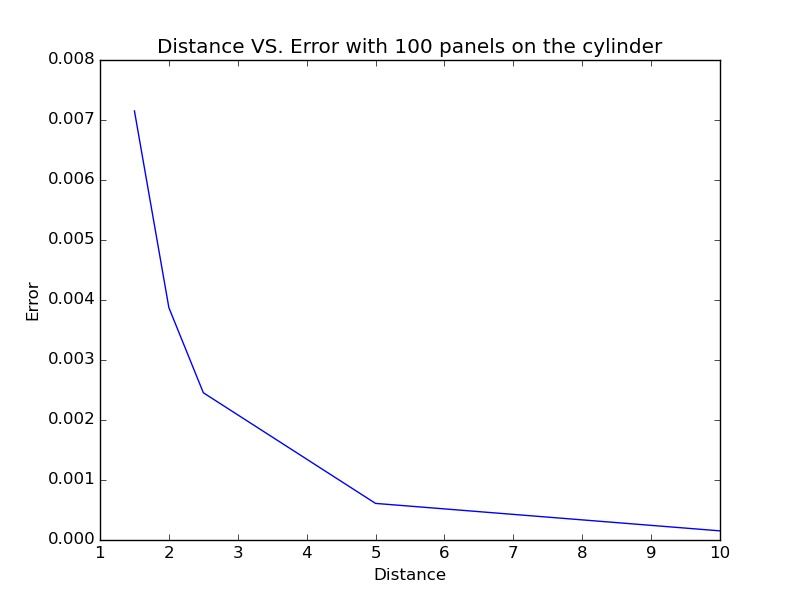
\includegraphics[width=12cm]{result3.jpg}
\caption{Error(relative average) Vs. Distance assuming 100 panels on the cylinder}
\label{figure:}
\end{figure}

\begin{figure}[H]  \label{figure}
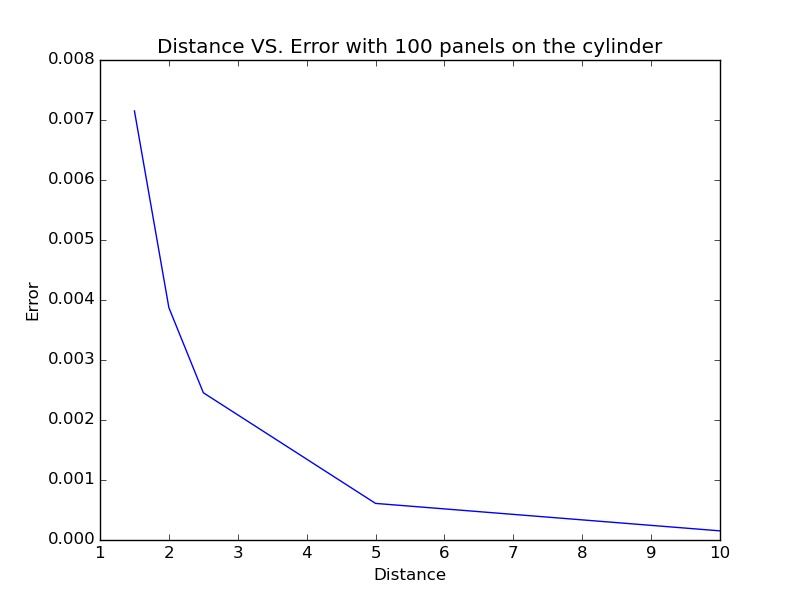
\includegraphics[width=12cm]{result3.jpg}
\caption{Error(relative average) Vs. Distance assuming 500 panels on the cylinder}
\label{figure:}
\end{figure}

Thus, it is clear that error decreases as the distance from the cylinder increases, since the effect of boundary condition decreases.
Error also decreses as the number of panels increases. 

\newpage
\section*{Question 3}
Consider the path of a single point vortex of strength 2 pi placed at a radius 1.5 units from the center of the cylinder of unit radius (without any free-stream). Integrate its path using the RK2 scheme. Also solve the same using the method of images and ensure that the paths are similar. Calculate the error.
\begin{figure}[H] \label{figure}
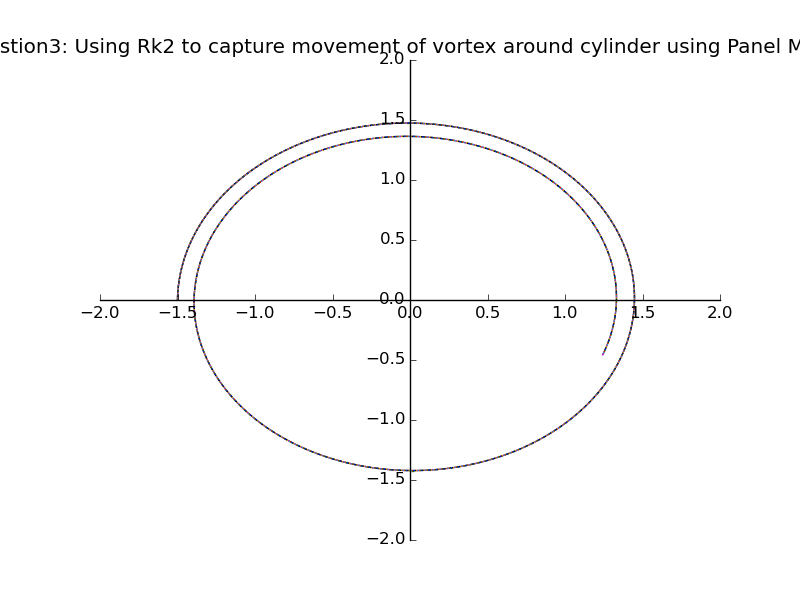
\includegraphics[width=12cm]{q3_panel.png}
\caption{Path Traced by Vortex kept at (0,1.5) using Panel approximation solution in 5 sec}
\label{figure:}
\end{figure}

\begin{figure}[H]  \label{figure}
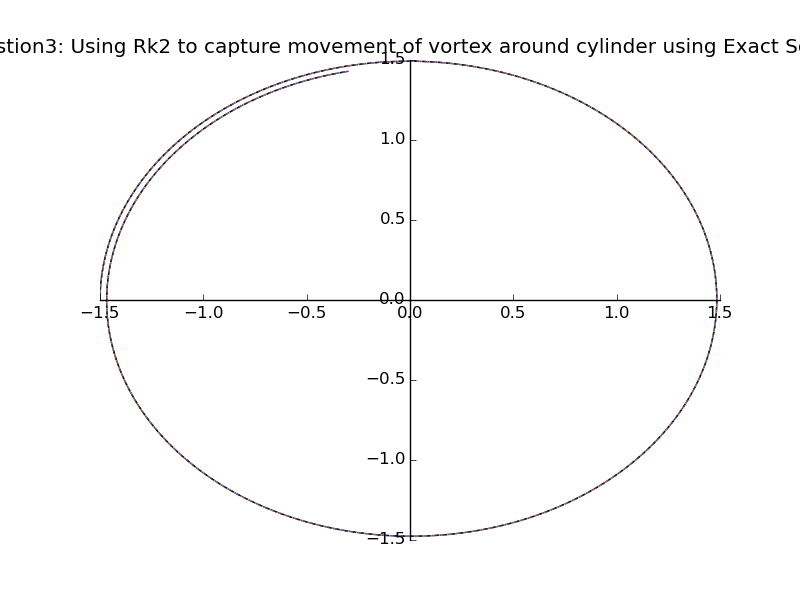
\includegraphics[width=12cm]{q3_exact.png}
\caption{Path Traced by Vortex kept at (0,1.5) using exact solution in 5 sec}
\label{figure:}
\end{figure}

Absolute Error in the final position the vortex after 5 sec = 0.292746493
Error Increases as the time increases.
 
  
\end{document}

